% Paper for the ChouchBase assignment.

\documentclass[]{IEEEtran}

\usepackage{float}
\usepackage{url}
\usepackage{graphicx}
\usepackage{color}

\begin{document}

\title{No Dogs On The Couch$_{Base}$}

% author names and affiliations
% use a multiple column layout for up to two different
% affiliations

\author{\IEEEauthorblockN{Eriq Augustine, Ryan Hnarkis, Aldrin Montana, Ryan Verdon, Tyler Yero}
\\
\IEEEauthorblockA{Department of Computer Science\\
Cal Poly, San Luis Obispo\\
 \textsf{\{eaugusti, rhnaraki, amontana, rverdon, tyero\}@calpoly.edu}
}
}

\maketitle

\thispagestyle{empty}
\pagestyle{empty}

\section{Introduction}\label{sec:introduction}
Gene annotation is the process of associating metadata about a gene with the
contig on which the gene resides. This metadata is necessary for conducting
genomic research projects and analysis involving the contig's genomic sequence.
Currently, there is no specifically gene annotation software. Genome browsers
all maintain lots of genomic data and are used to be able to annotate genes and
contigs, but do not provide a user-friendly interface. While genome browsers
will likely never be replaced (UCSC genome browser, etc. are well
established), it would be desirable to have a software system that better
accomodates the visual and informational needs of gene annotation.

\textit{CGAT} is a web-based gene annotation application designed with
usability, simplicity, and efficiency in mind. It is not a feature and data
rich genome browser like the \textit{UCSC genome brower}. Nor is \textit{CGAT}
designed to be a replacement for other genome browsers in any aspect other than
gene annotation. Other gene browsers attempt to accommodate many needs of the
biology community and so offer many features, and a cluttered, chaotic
interface. Gene annotation, while not a trivial task, can be well-serviced by a
simple data model. Ideally, by focusing on a simple data model, \textit{CGAT}
is able to provide a clean, streamlined experience. \textit{CGAT} aims to
provide users with a way to view gene annotations without extra, unnecessary
information obscuring their view while also embodying a wikipedia-like emphasis
on collaboration and openness.

Anya Goodman, a professor in the biochemistry department at Cal Poly, San Luis
Obispo, offers a bioinformatics course that covers several aspects of gene
annotation. This project is spearheaded by Ryan Verdon to accommodate Dr.
Goodman's needs and ideas for ideal gene annotation software.

This paper primarily focuses on considerations for \textit{CGAT}'s database
architecture. These considerations are made with regards to a MySQL cluster
versus a Couchbase cluster to determine what database architecture is most
efficient for running \textit{CGAT}. Section \ref{sec:motive} discusses our
motivation to compare couchbase and MySQL in this paper, while section
\ref{sec:design} talks about how we designed experimental workloads to use for
our comparison of couchbase vs MySQL. In section \ref{sec:workload} we
describe the workloads and how they are relevant to \textit{CGAT}, some brief
implementation details are outlined in section \ref{sec:implementation}, we
evaluate our results in section \ref{sec:eval} and finally conclude in
section \ref{sec:conclusions}.

\section{Motivation}\label{sec:motive}
To evaluate the performance we auto-generated around
400MB of data and inserted the same data into each cluster.  Obviously using a
different data model for Couchbase to accommodate for the fact it is a NoSQL
key-value store instead of a relational database. We then created a set of six
experiments to run. Five came from common use cases found in the web
application. While the other was designed to test the performance on each
cluster of repeatedly writing and reading from the same object. Our major
metrics are write performance, read performance, and time-delay between writes
and reads of the same data. The rest of the paper is broken down as follows.
Section 2 describes in depth how we designed the experiment. Section 3
discusses the workloads we ran on each system. Section 4 describes our
implementation.  Section 5 goes into the results of each of our experiments and
some analysis on the data we obtained. Lastly, section 6 presents our
conclusions.
 
\section{Experiment Design}\label{sec:design}
For our experiments we are using a total of five EC2 instances from the Amazon
Web Services cloud. For both of our systems four servers were used for the
database while the last was used for running our workload harness. The MySQL
system is setup with one master server for writes and three slaves servers that
replicate all of the masters data. Unlike the Couchbase system where each
server handled a subset of the data.

Our major driving force of this experiment was to see how Couchbase compared to
MySQL for running a web application. To test which is better we created a
workload harness. The main tasks of the workload harness was to define how many
times a workload would run and which workloads to run. In our case workloads
define a certain task. For example, getting of the data necessary to display a
users profile. In our system a workload knows how to do its job in both MySQL
and the Couchbase API. We leave describing each type workload we ran to the
next section.

As each workload is run the workload harness records important stats. Some of
the stats include how long the workload took to run, the min and max times of
an individual query or insertion, and the standard deviations of individual
runs.

\subsection{Data}
The data we are storing comes from Ryan Verdon's masters thesis. It is the
backend for a community genome annotation database. It contains data like
genome sequences, genes, and species information. The representation of the
data is vastly different in the two systems. 

But there exists four main pieces of data that are crucial to either
representation. They are contigs, annotations, users, and groups. Contigs are
what a biologist annotates to find genes. The main portion of a contig is a DNA
sequence. Annotations are the record or formal representation of a gene that
has been found in a specific contig. An annotation has several parts including
coordinates in the contig which specify individual exons and meta information
about the annotation like who uploaded it and when it was done, etc. 

Groups are another important part of the usefulness of the system. Users of
like minds can join the same group to receive important information. Users is a
major part of the data and is one of the central pillars that connects the
data. Users upload contigs, create annotations, and join groups. Below we show
the different ways we store the data in SQL and JSON.

\subsubsection{SQL}
In SQL the data is represented as nine tables. A diagram of the tables with
links to represent foreign key constraints is shown in Figure 1. 

\subsubsection{JSON}
For Couchbase we used four JSON objects which are shown in Figures 2-5. We left
out the JSON object for the test table. It just consisted of two fields (Id and
Name). All of the information from the SQL tables is represented in these JSON
objects. We take advantage of nested objects to reduce as much subsequent
requerying of the database as possible.

\begin{figure}
	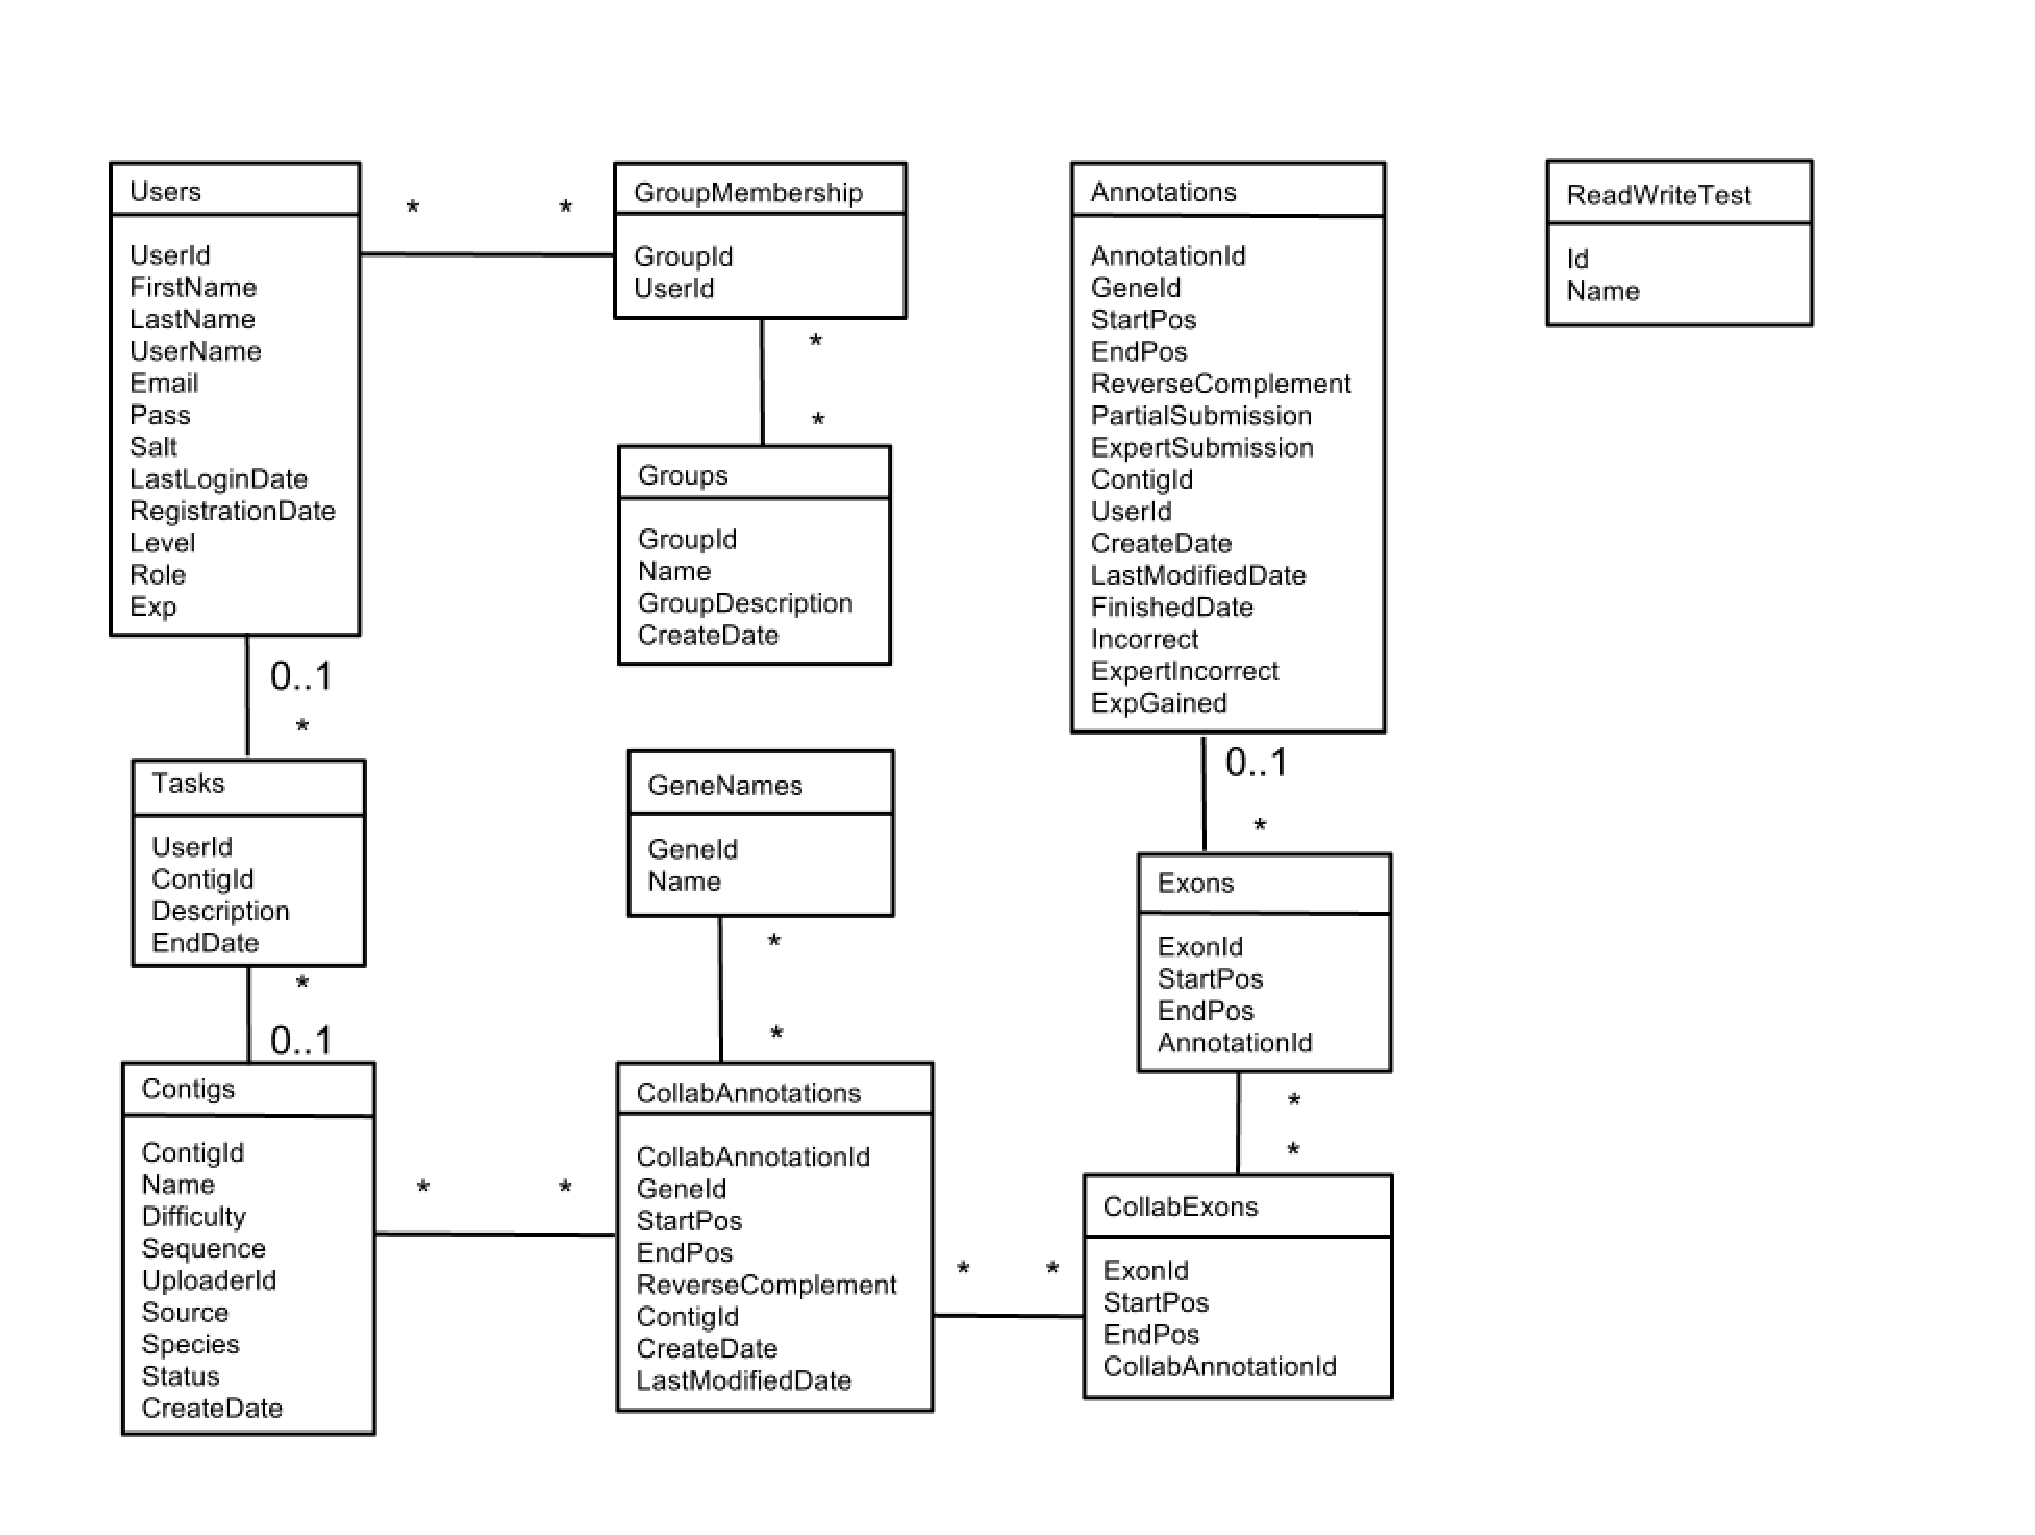
\includegraphics[width=5.5in]{SQLDiagram.eps}
	\caption{The SQL diagram for CGAT.}
	\label{fig:SQLDiagram}
\end{figure}

%\clearpage

\begin{figure}%
	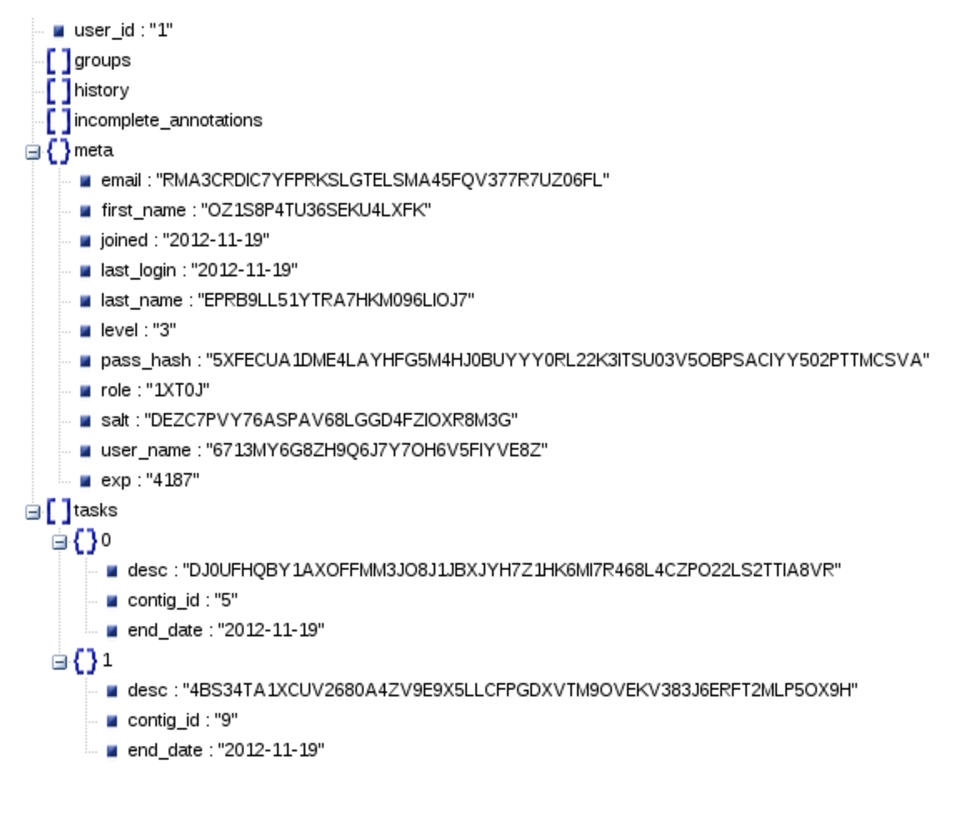
\includegraphics{user.eps}
	\caption{The JSON for a user.}
	\label{fig:JSON-user}
\end{figure}%

\begin{figure}%
	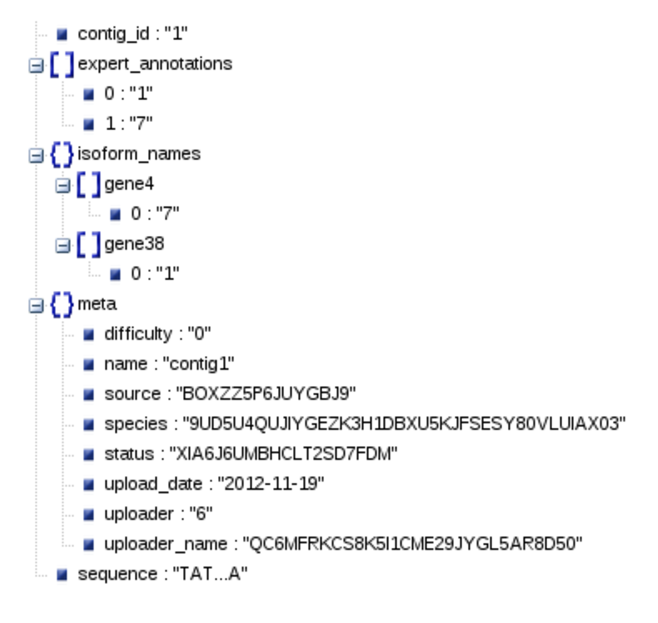
\includegraphics[height=70mm]{contig.eps}
  \caption{The JSON for a contig.}
  \label{fig:JSON-contig}
\end{figure}%

\begin{figure}%
	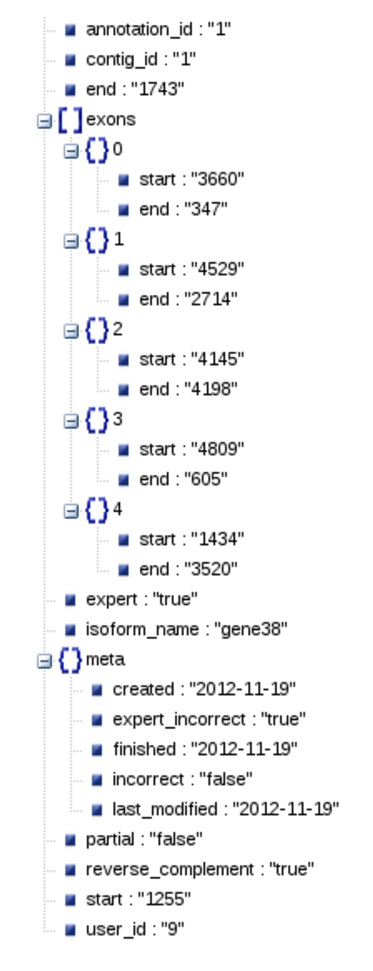
\includegraphics[height=100mm]{annotation.eps}
	\caption{The JSON for an annotation.}
	\label{fig:JSON-annotation}
\end{figure}%

\begin{figure}%
	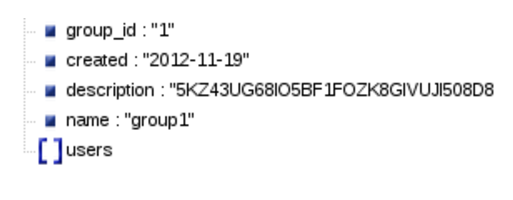
\includegraphics[height=20mm]{group.eps}
	\caption{The JSON for a group.}
	\label{fig:JSON-group}
\end{figure}%

\clearpage

\section{Workloads}\label{sec:workload}
The core unit of work that we used to compare couchbase performance against
MySQL performance was called a \textit{workload}. Each workload was designed
either to be write-heavy, read-heavy, or balanced. The number of workloads used
during our comparison was determined by the number of members in our group (as
specified by Alex Dekhtyar). Unfortunately due to time constraints we were
unable to do multiple runs of any one workload, however, due to our environment
and machines, there should be minimal fluctuations in any given run time for a
workload.

In this section we further describe each task's purpose as well as what type of
workload it was (write-heavy, etc.). This is necessary to be able to properly
interpret (and agree or disagree with) the results described in section
\ref{sec:eval}.

\subsection{Profile View}
The first thing that all users will do in \textit{CGAT} (ideally) is log in.
When a user logs into \textit{CGAT} the user will be directed to his profile
view which will contain all groups they are a member of, all completed
annotations they have submitted, partial annotations that have been saved, and
all tasks they have assigned. This is a use case that is likely to see many
additions in the future as it serves as the first and foremost view of the
system for the user. This means that any information that should be accessible
-- including when a forum system is integrated into \textit{CGAT} -- will find
a place on the user's profile.

This workload is clearly a read-heavy workload that entails no disk writes at
all. Important to note though, this use case may constantly be increasing
(should constantly be increasing for a successful system) and so the load for
this workload may increase quite a bit, and whenever new features are added
there is a potential for a spike in workload.

%TODO make sure overview of CGAT defines what a task is, and mentions user
%groups
\subsection{Task Assignment}
In \textit{CGAT}, it must be possible to request a group of users to annotate
new or updated contigs. The frequency of this use case is dependent on the
adoption of \textit{CGAT} -- the more species \textit{CGAT} supports, the more
frequent this use case will be. More specifically, the relevant entities in the
\textit{CGAT} schema are \textit{users}, \textit{contigs}, and \textit{groups}.
Since a task embodies a request for a group $G$ to annotate a contig $C$, every
user $U$ in $G$ receives a notification including a description of $C$ and a
message requesting that it be annotated. A task can be assigned to any number
of groups. Since tasks are assigned to groups that have some vested interest in
the species or specific contig that has been updated or added, there may be
many groups that a task should be assigned to. Additionally, as more species
are supported by \textit{CGAT} or more users join \textit{CGAT}, more users
will receive notifications of tasks and so there are multiple ways in which
this use case must be scalable.

This workload is write-heavy -- adding tasks for each user in a group requires
adding many records to a relational table or modifying many documents/values
in a key/value store.

%TODO make sure overview of CGAT mentions experience, and defines what an
%annotation is
\subsection{Annotation Publication}
Annotations are the core focus of \textit{CGAT}. Every user is going to be
doing some annotation, and they should be doing many annotations. Especially
since \textit{CGAT} defines an annotation to be information about a gene
isoform on a contig, even annotating a single gene will yield to several
annotations in \textit{CGAT}. Additionally, when an annotation is submitted,
the annotation must be marked as complete, the user and annotation then are
assigned a certain amount of experience--the user gains experience towards
his total, the annotation gains experience and serves as a history of the
user's experience.

This is a mostly write-, somewhat read-heavy workload. It is write-heavy in the
sense that it must update a user and the annotation that the user completed.
However, it also has some reads in the sense that the contig, for which the
annotation is being submitted, is used to determine the amount of experience
that submitting the annotation yields for the user. However, given the
difference in data model between couchbase and MySQL, the couchbase
implementation is much more write-heavy than the SQL equivalent. This is
because the couchbase data model includes lists of complete and incomplete
annotations for each user so that the annotation does not have to be fetched
for every use case involving users and annotations. Since this is the case,
more of the document undergoes modification for this use case (though I'm not
sure if couchbase optimizes its writes in a way that many modifications in the
same document is slower than few modifications in the same document).

\subsection{Group Membership Modification}
Group membership is likely the second most stable of the workloads used in our
comparisons of couchbase vs MySQL next to contig uploads. This is ``stable''
because the majority of users will only join groups, and leaving groups will
likely be relatively rare. This use case will only ever be as bad as how many
users join at any one time--once a user registers for \textit{CGAT} and has
joined some groups the user is unlikely to join or leave groups and so this use
case poses almost no scalability problems. Although, despite this, there will
be spikes that coincide with academic schedules, as groups will be created and
populated for each new class that uses \textit{CGAT}.

This workload is the most balanced of the workloads described in this paper
(except maybe for ``stupid'' workload). Generally speaking, when a user joins a
group then there is only the addition of a record in MySQL or the modification
of the user document in couchbase. And when a user leaves a group, then
subsequently the additional relational tuple or field in the user document is
``undone'' by removing the group membership tuple or deleting the field from
the user document. 

\subsection{Contig Uploads}
Contig uploads is the most stable workload when the manual, or user, use case
is considered. Although, there will be large spikes of activity when/if the
reference genome for a species is updated--requiring \textit{CGAT} to update
any and all of the contigs relevant to the genome. However, reference genomes
are updated very infrequently and contigs will never be removed from
\textit{CGAT}.

This workload is write-heavy because it requires no reads--the use case is for
uploading data, not downloading data.

\subsection{Stupid}
This is a test workload to examine the performance of writing and reading from
the same object in succession. This is a workload contrived purely for better
comparison of couchbase vs MySQL instead of workloads representative of what
\textit{CGAT} will rely on. This is a naive, balanced workload.

\section{Implementation}\label{sec:implementation}
Our experiment was implemented completely in Java. To do the MySQL portion of
the workload we used the MySQL JDBC driver. For the Couchbase portion we used
the Couchbase Java library from their website.

\section{Evaluation}\label{sec:eval}
In this section we discuss the results from each workload in turn.

%section on each workload and the results on each system (could be a table tbh and not a graph)
%probably some weak analysis on why we expected the results
%need to ask eriq the # of times each workload was  run, might be in an email?

\subsection{Assigning a Task}

\subsection{Profiling}

\subsection{Publishing}

\subsection{Adding and Removing Group Membership}

\subsection{Uploading Contigs}

\subsection{Read and Writing Performance}

\section{Conclusions}\label{sec:conclusions}
TODO

% TODO: Uncomment if we use any refs
% \bibliographystyle{acm}
% \bibliography{refs}

\end{document}
